\chapter{Lec 13 - Resolution for First Order Logic}

\section{Resolution}
The last of our three families of logical systems is based on \textbf{resolution}. In resolution for first order logic two clauses, which are assumed to be standardized apart so
that they share no variables, can be resolved if they contain complementary literals. Propositional literals are complementary if one is the negation of the other; first-order literals are complementary if one unifies with the negation of the other. Thus, we have
\begin{center}
    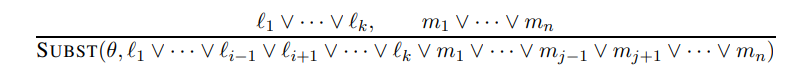
\includegraphics[]{images/resolution-fol.png}
\end{center}
where $UNIFY(l_i,\neg{m_j} ) = \theta$. For example, we can resolve the two clauses
\[[Animal(F(x)) \lor Loves(G(x), x)]\,\, \text{and} \,\,[\neg Loves(u, v) \lor \neg Kills(u, v)]\]
by eliminating the complementary literals $Loves(G(x), x)$ and $\neg Loves(u, v)$, with unifier $\theta = \{u/G(x), v/x\}$, to produce the \textbf{resolvent} clause
\[[Animal(F(x)) \lor \neg Kills(G(x), x)] .
\]
Then, the resolution steps can be applied to $CNF(KB \land \neg \alpha)$ as we did for propositional logic.

\section{Conversion to CNF}
As in the propositional case, first-order resolution requires that sentences be in \textbf{conjunctive
normal form} (CNF), that is, a conjunction of clauses, where each clause is a disjunction of literals. Literals can contain variables, which are assumed to be universally quantified. Every sentence of first-order logic can be converted into an inferentially equivalent CNF
sentence.\\\\
We illustrate the procedure by translating the sentence “Everyone who loves all animals is loved by someone,” or
\[\forall x \, [\forall y \, Animal(y) \Rightarrow Loves(x, y)] \Rightarrow [\exists y \, Loves(y, x)].\]
The steps are as follows:
\begin{itemize}
    \item \textbf{Eliminate implications:}
    \[\forall x \, [\neg \forall y \, \neg Animal(y) \lor Loves(x, y)] \lor [\exists y \, Loves(y, x)] .\]

    \item \textbf{Move} $\neg$ \textbf{inwards}: In addition to the usual rules for negated connectives, we need rules for negated quantifiers. Thus, we have
    \[\begin{split}
        & \neg \forall x \, p \,\, \text{becomes} \,\, \exists x \, \neg p\\
        & \neg \exists x \, p \,\, \text{becomes} \,\, \forall x \, \neg p .
    \end{split}\]
    Our sentence goes through the following transformations:
    \[\begin{split}
        & \forall x \, [\exists y \, \neg(\neg Animal(y) \lor Loves(x, y))] \lor [\exists y \, Loves(y, x)].\\
        & \forall x \,[\exists y \, \neg \neg Animal(y) \land \neg Loves(x, y)] \lor [\exists y \, Loves(y, x)].\\
        & \forall x \,[\exists y \, Animal(y) \land \neg Loves(x, y)] \lor [\exists y \, Loves(y, x)]
    \end{split}
    \]

    \item \textbf{Standardize variables}: each quantifier should use a different one:
    \[\forall x \,[\exists y \, Animal(y) \land \neg Loves(x, y)] \lor [\exists z \, Loves(z, x)] .\]

    \item \textbf{Skolemize:} \textbf{Skolemization} is the process of removing existential quantifiers by elimination. In the simple case, it is just like the Existential Instantiation rule seen previously: translate $\exists x \, P(x)$ into $P(A)$, where $A$ is a new constant. However, we can’t apply Existential Instantiation to our sentence above. If we blindly apply the rule to the two matching parts we get
    \[\forall x \, [Animal(A) \land \neg Loves(x, A)] \lor Loves(B,x),\]
    which has the wrong meaning entirely: it says that everyone either fails to love a particular animal $A$ or is loved by some particular entity $B$. Thus, we want the Skolem entities to depend on $x$ and $z$:
    \[\forall x \, [Animal(F(x)) \land \neg Loves(x, F(x))] \lor Loves(G(z), x) .\]
    Here $F$ and $G$ are \textbf{Skolem functions}.  The general rule is that the arguments of the Skolem function are all the universally quantified variables in whose scope the existential quantifier appears.

    \item \textbf{Drop universal quantifiers:}  At this point, all remaining variables must be universally quantified. Moreover, the sentence is equivalent to one in which all the universal quantifiers have been moved to the left. We can therefore drop the universal quantifiers:
    \[[Animal(F(x)) \land \neg Loves(x, F(x))] \lor Loves(G(z), x) .\]


    \item \textbf{Distribute} $\lor$ \textbf{over} $\land$:
    \[[Animal(F(x)) \lor Loves(G(z), x)] \land [\neg Loves(x, F(x)) \lor Loves(G(z), x)].\]
\end{itemize}
The sentence is now in CNF and consists of two clauses.

\section{Example proofs}
Resolution proves that $KB \vDash \alpha$ by proving $KB \land \neg \alpha$ unsatisfiable, that is, by deriving the empty clause. The algorithmic approach is identical to the propositional case. We give two example proofs. The first is the crime example presented in the previous sections. The sentences in CNF are:
\begin{center}
    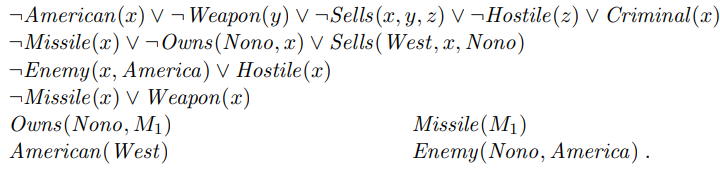
\includegraphics[]{images/crime-cnf.png}
    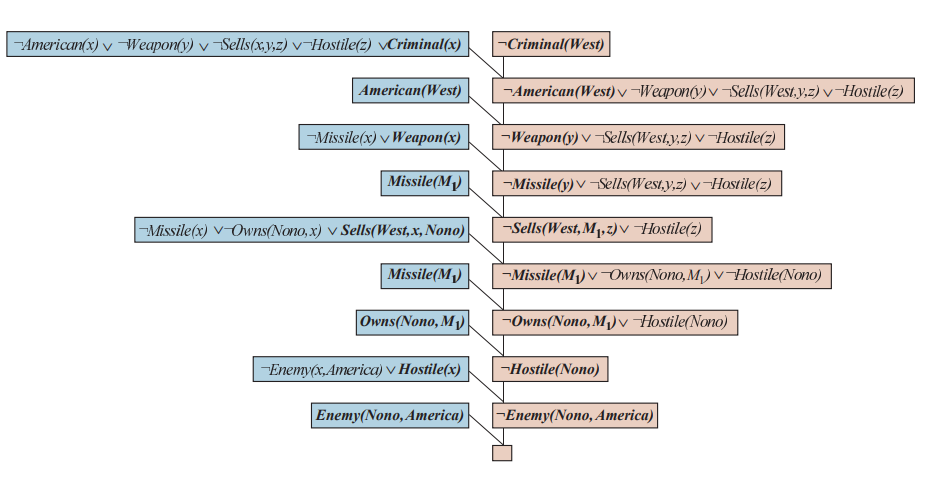
\includegraphics[]{images/resolution-crime-fol.png}
\end{center}
The resolution proof is shown in the figure above. Notice the structure: single “spine” beginning with the goal clause, resolving against clauses from the knowledge base until the empty clause is generated. This is characteristic
of resolution on Horn clause knowledge bases. In fact, the clauses along the main spine correspond exactly to the consecutive values of the goals variable in the backward-chaining algorithm.\\\\
Our second example makes use of Skolemization and involves clauses that are not definite clauses. This results in a somewhat more complex proof structure. In English, the problem is as follows:
\begin{center}
    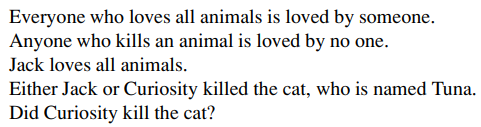
\includegraphics[]{images/resolution-fol-proof.png}
\end{center}
First, we express the original sentences, some background knowledge, and the negated goal G in first-order logic:
\begin{center}
    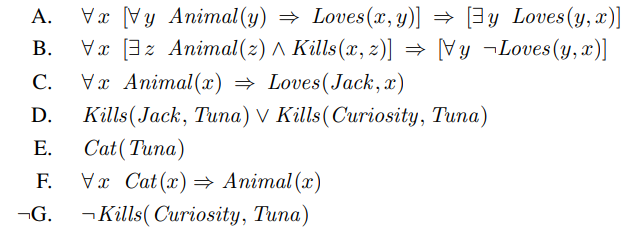
\includegraphics[]{images/kb-res-proof.png}
\end{center}
Now we apply the conversion procedure to convert each sentence to CNF:
\begin{center}
    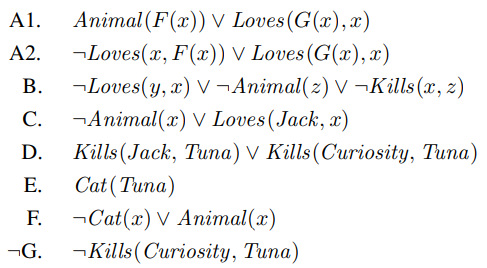
\includegraphics[]{images/kb-cnf-re-prrof.png}
\end{center}
The resolution proof that Curiosity killed the cat is given in the figure below:
\begin{center}
    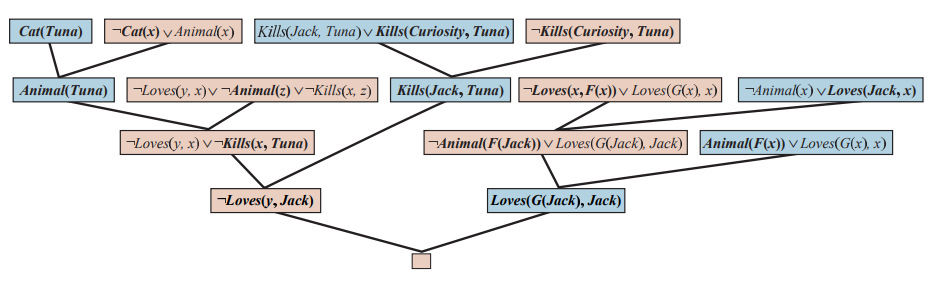
\includegraphics[]{images/res-proof-tree.png}
\end{center}
The proof answers the question “Did Curiosity kill the cat?” but often we want to pose more general questions, such as “Who killed the cat?”. Then, the goal is $\exists w \, Kills(w, Tuna)$, which, when negated, becomes $\neg Kills(w, Tuna)$ in CNF. Repeating the proof with the new negated goal, we obtain a similar proof tree, but with the substitution {w/Curiosity} in one of the steps. Unfortunately, resolution can produce \textbf{nonconstructive proofs} for existential goals. For example, $\neg Kills(w, Tuna)$ resolves with $Kills(Jack, Tuna) \lor Kills(Curiosity, Tuna)$ to give $Kills(Jack, Tuna)$, which resolves again with $\neg Kills(w, Tuna)$ to yield the empty clause. Notice that $w$ has two different bindings in this proof; resolution is telling us that, yes, someone killed Tuna, either Jack or Curiosity. This is no great surprise!
\begin{center}
    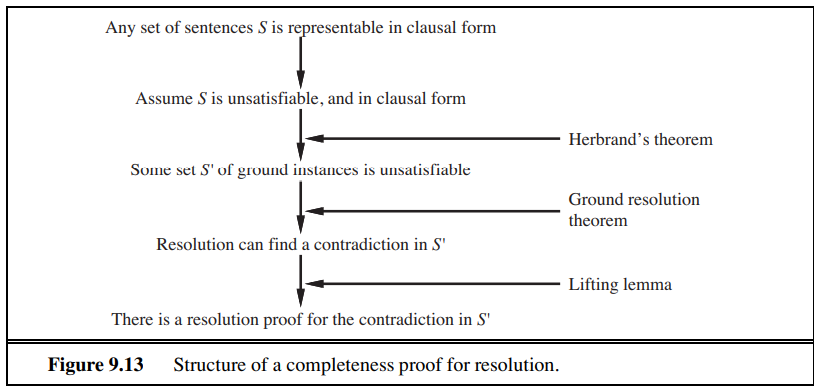
\includegraphics[]{images/res-completeness-fol.png}
\end{center}

\section{Resolution strategies}
We know that repeated applications of the resolution inference rule will eventually find a proof if one exists. In this subsection, we examine strategies that help find proofs efficiently.
\begin{itemize}
    \item \textbf{Unit preference/clause}: prefers to do resolutions where one of the sentences is a single literal.  The idea behind the strategy is that we are trying to produce an empty clause, so it might be a good idea to prefer inferences that produce shorter clauses.

    \item \textbf{Unit resolution:} is a restricted form of resolution in which every resolution step \textbf{must} involve a unit clause. Unit resolution is incomplete in general, but complete for Horn clauses. Unit resolution proofs on Horn clauses resemble forward chaining.

    \item \textbf{Set of support:} every resolution step involve at least one element of a special set of clauses (the set of support); the resolvent is then added into the set of support. Incomplete if the wrong set of support is chosen.

    \item \textbf{Input resolution:} In this strategy, every resolution combines one of the input sentences (from the KB or the query) with some other sentence. Complete for knowledge bases that are in Horn form, but incomplete in the general case. Input resolution has the characteristic shape of a single “spine” with single sentences combining onto the spine. The \textbf{linear resolution} strategy is a slight generalization that allows $P$ and $Q$ to be resolved together either if $P$ is in the original KB or if $P$ is an ancestor of $Q$ in the proof tree. Linear resolution is complete.

    \item \textbf{Subsumption:} eliminates all sentences that are subsumed by (that is, more specific than) an existing sentence in the KB. For example, if $P(x)$ is in the KB, then there is no sense in adding $P(A)$ and even less sense in adding $P(A) \lor Q(B)$. Subsumption helps keep the KB small and thus helps keep the search space small.

\end{itemize}
